\documentclass[11pt,letterpaper]{article}
\usepackage{fullpage}

\usepackage[english]{babel}
\usepackage[utf8]{inputenc}
\usepackage{amsmath}
\usepackage{graphicx}
\usepackage[hidelinks]{hyperref}
\usepackage{float}
\usepackage{amsfonts}
\usepackage{algorithm,algpseudocode}
             
\graphicspath{{../results}}
             
\begin{document} 

\title{Experiment 2}
\maketitle

\section*{Differences from Experiment 1}

The only difference between this experiment and experiment 1 is that we give principal 2 a ``headstart" in the sense of letting them be the only firm in the market for the first 1000 periods. Thus, the principals are effectively given 1000 free observations for learning and the agents are given 1000 free observations in order to form a reputation score for principal 2. The question this simulation then attempts to answer is if \textit{information advantage} can be viewed as a barrier to entry. Namely, it attempts to begin to answer if the first mover advantage manifests itself in this model by giving the incumbent firm a better prior than any entrants (who we assume come in with only ``fake" priors). Under what assumptions about the agent rationality (response functions or memory sizes) and what algorithms do we see the entering firm able to gain any market share?
\section*{Simulation Details}

Considered $K = 3$, $T = 5005$, $N = 60$. Report statistics at $t = 1000, 3000, 5000$ \\
\textbf{The Bandit priors that were considered}:
\begin{itemize}
\item Uniform: Draw the mean rewards for the arms from [0.25, 0.75]
\item ``HeavyTail": We took the mean rewards to be randomly drawn from Beta($\alpha=0.6,\beta=0.6$). With this distribution it was likely to have arms that were at the extremes (close to 1 and close to 0) but also some of the arms with intermediate value means.
\item Needle-in-haystack
\begin{enumerate}
\item Medium - 9 arms with mean 0.50, 1 arm with mean 0.55 (+ 0.05)
\item High - 9 arms with mean 0.50, 1 arm with mean 0.70 (+ 0.20)
\end{enumerate}
\end{itemize}
\textbf{Algorithms considered}:
\begin{enumerate}
\item ThompsonSampling with priors of $Beta(1, 1)$ for every arm.
\item DynamicGreedy with priors of $Beta(1, 1)$ for every arm
\item Bayesian Dynamic $\epsilon$-greedy with priors of $Beta(1, 1)$ for every arm and $\epsilon=0.05$
\end{enumerate}
\textbf{Agent Algorithms considered}:
\begin{enumerate}
\item HardMax
\item HardMaxWithRandom
\item SoftMax
\end{enumerate}
\textbf{Memory Sizes}
\begin{enumerate}
\item 10
\item 25
\item 100
\end{enumerate}

The simulation procedure is the only thing that has changed compared to Experiment 1:
\textbf{Simulation Procedure}
\begin{algorithm}[H]
\begin{algorithmic}[1]
\For{Each prior $p$}
	\For{Each agent algorithm $agent alg$}
		\For{Each principal algorithm pair $principalalg1$, $principalalg2$}
			\For{$N$ simulations}
				\State Generate true distribution from $p$ (except for needle-in-haystack, just use $p$ itself)
				\State Give the agents 5 observations from each principal
				\State Give principal 2 1000 free observations (and give the agents this information too)
				\State Run simulation for T periods
			\EndFor
		\EndFor
	\EndFor
\EndFor
\end{algorithmic}
\end{algorithm}

\pagebreak
\section*{Results}
\textbf{HardMax} \\
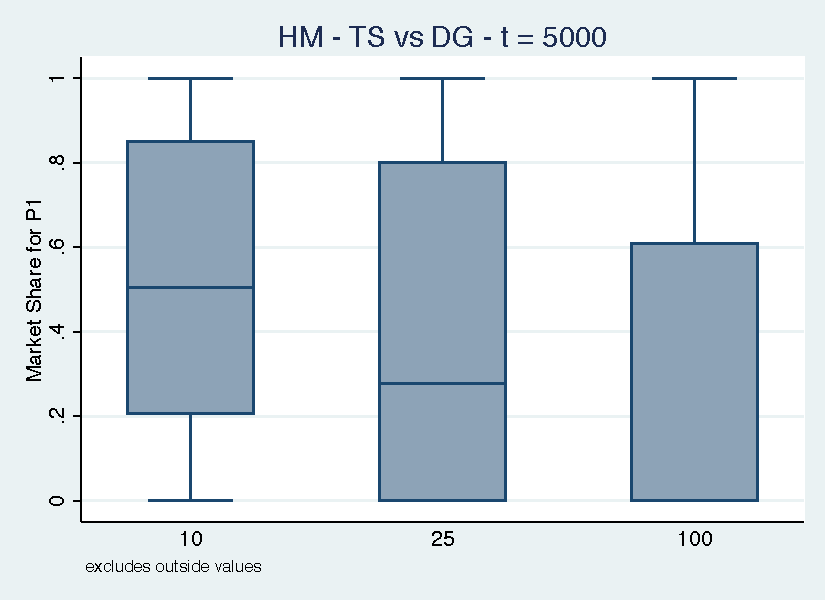
\includegraphics[scale=0.9]{hm_ts_dg_memory_5000} \\ 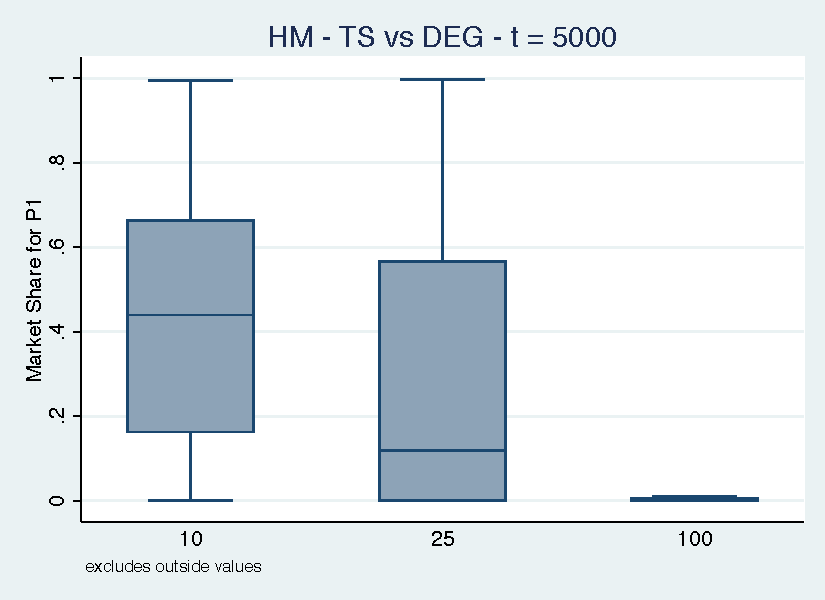
\includegraphics[scale=0.9]{hm_ts_deg_memory_5000} \\
The main interesting result here is that for ThompsonSampling vs DEG, with low memory sizes we have that ThompsonSampling almost catches up to DEG, but as we increase memory size TS gets almost no market share! Should re-run this experiment with higher N to validate this. 

\pagebreak
\textbf{HardMaxWithRandom}  \\
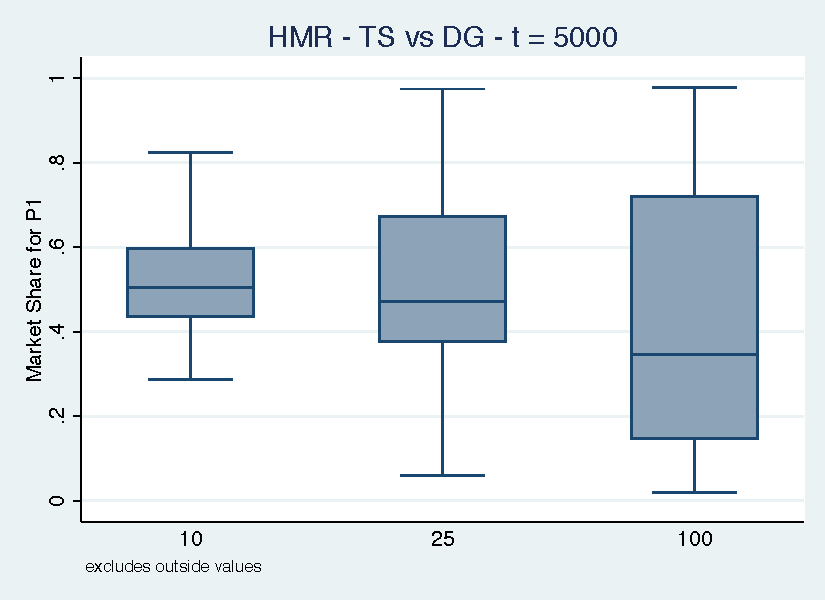
\includegraphics[scale=0.9]{hmr_ts_dg_memory_5000} \\ 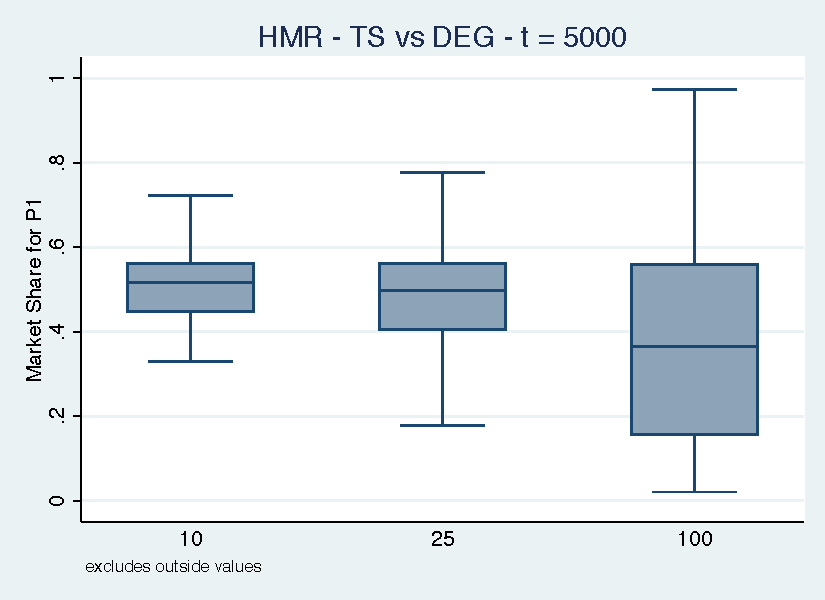
\includegraphics[scale=0.9]{hmr_ts_deg_memory_5000}

\pagebreak
\textbf{SoftMax} \\
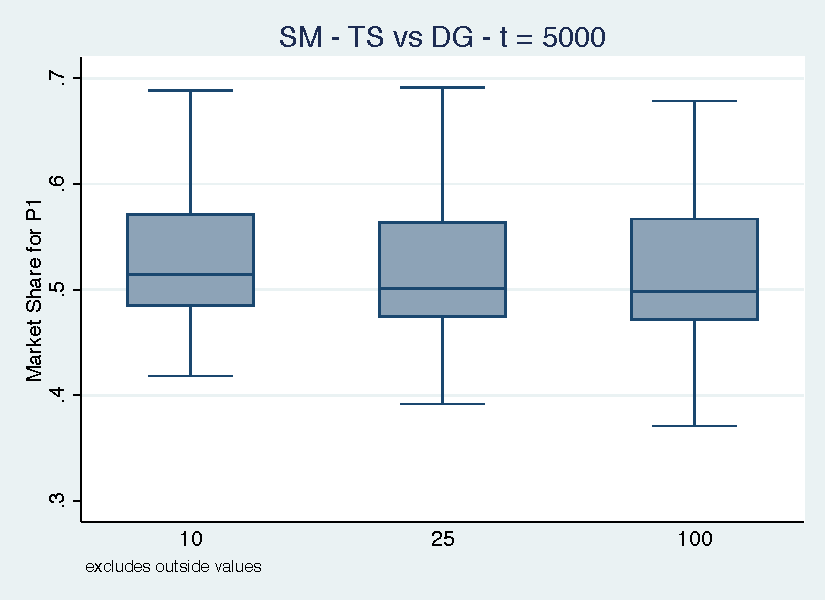
\includegraphics[scale=0.9]{sm_ts_dg_memory_5000} \\ 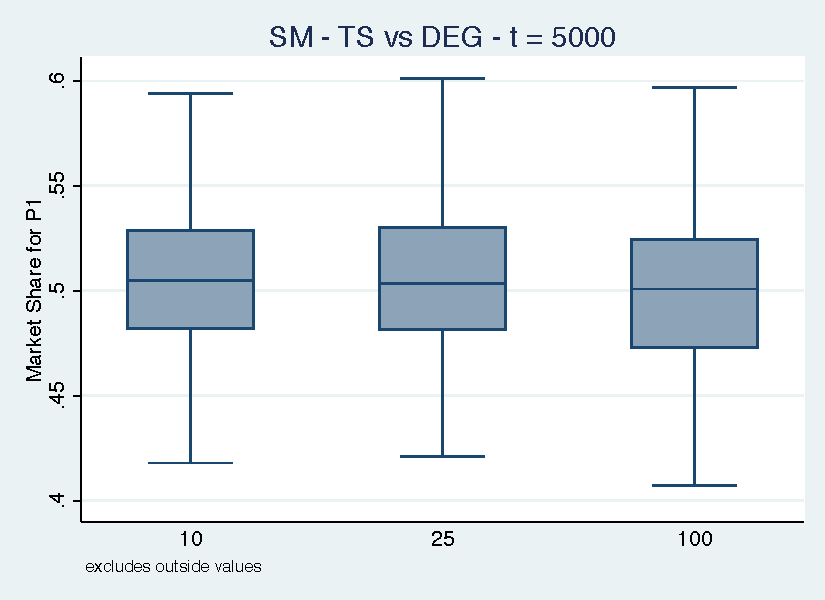
\includegraphics[scale=0.9]{sm_ts_deg_memory_5000}

\pagebreak
Zooming in on the HardMax results and looking at them over time we get (for memory = 25): \\
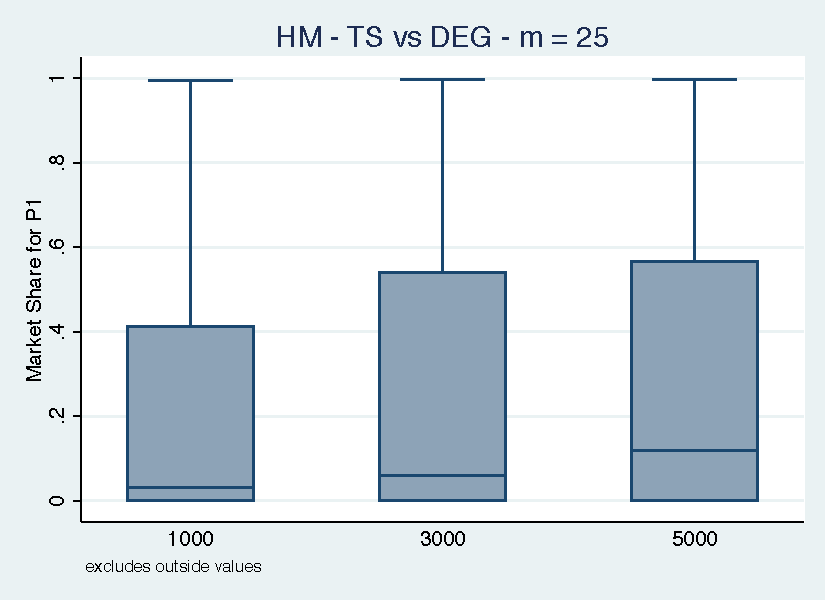
\includegraphics[scale=0.9]{hm_ts_deg_25_timehorizon} \\ 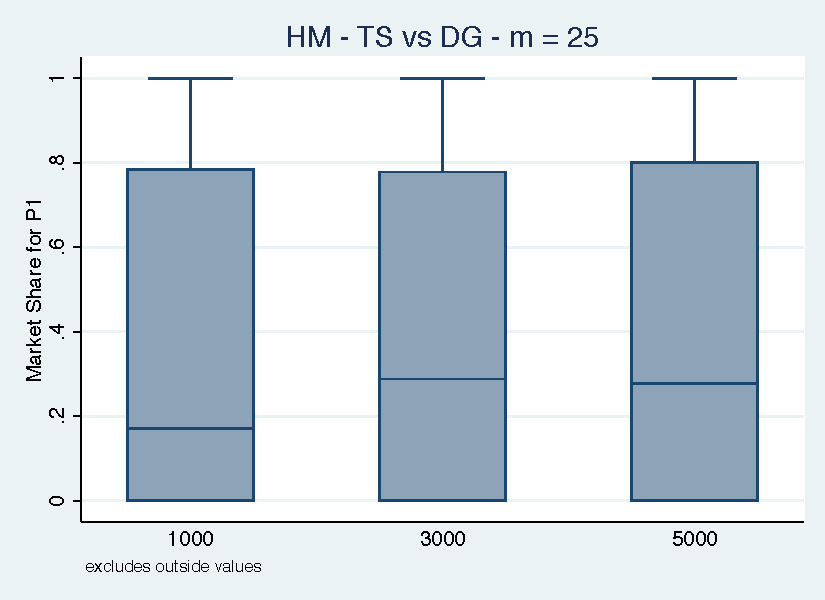
\includegraphics[scale=0.9]{hm_ts_dg_25_timehorizon}

\pagebreak
\textbf{Memory = 100} \\
Take note of the scale on the y-axis on this graph. \\
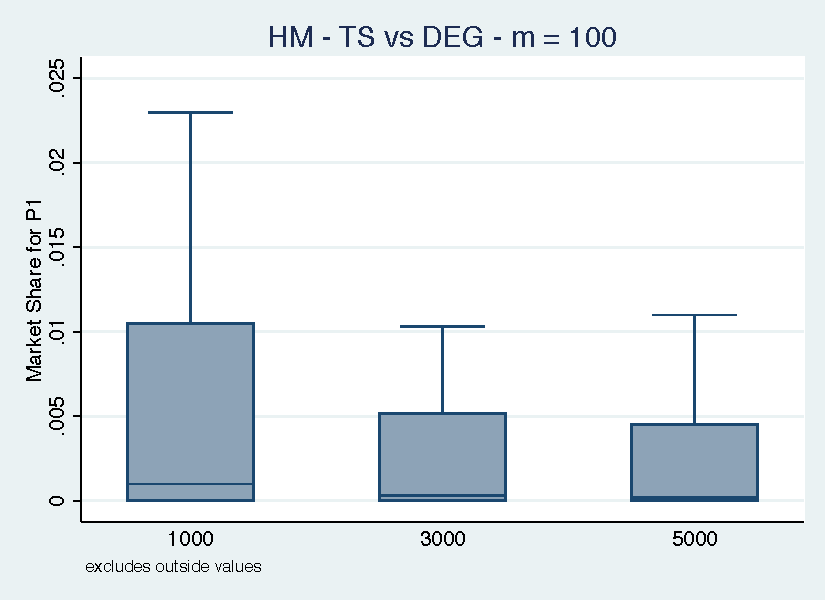
\includegraphics[scale=0.9]{hm_ts_deg_100_timehorizon} \\ 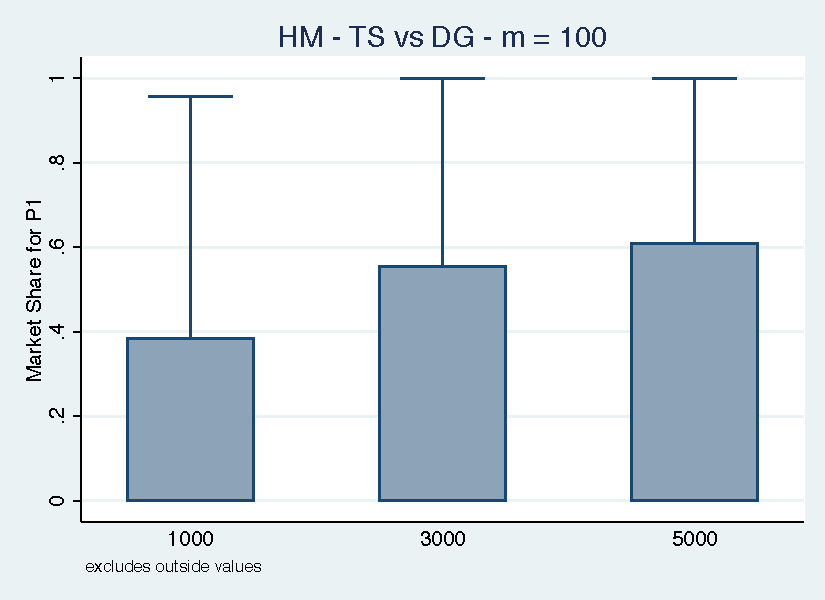
\includegraphics[scale=0.9]{hm_ts_dg_100_timehorizon}




\end{document}